\documentclass[11pt,a4paper,twoside,openright]{report}

%frontespizio
\providecommand{\coursename}{Progetto di Ingegneria Informatica}
\providecommand{\annoacc}{2013-2014}
\providecommand{\principaladviser}{Prof. Andrea Bonarini}
\providecommand{\firstauthor}{Davide Tateo}
\providecommand{\firstauthorid}{799311}
\title{Cognitive SLAM: Knowledge-Based Simultaneous Localization and Mapping}
\author{\firstauthor}

\usepackage{settings/frontesp}

\usepackage[italian]{hyperref}
\hypersetup{
    colorlinks,
    citecolor=black,
    filecolor=black,
    linkcolor=black,
    urlcolor=black
}
\newcommand{\autorefA}[1]{\hyperref[#1]{Algoritmo \ref{#1}}}

\usepackage{tabularx}
\usepackage{subfigure}
\usepackage{afterpage}
\usepackage{amsmath,amssymb}
\usepackage{amsthm}
\usepackage{rotating}  
\usepackage{fancyhdr}
\usepackage{algorithm}
\usepackage{algorithmic}
\usepackage[epsilon]{backnaur}
\usepackage[nottoc,notlot,notlof]{tocbibind}
\usepackage[scriptsize]{caption} 

\setlength{\oddsidemargin} {2. cm}
\setlength{\evensidemargin} {2. cm}
\addtolength{\oddsidemargin} {-0.4 cm}
\addtolength{\evensidemargin} {-0.4 cm}
\linespread{1.1}

\usepackage[italian]{babel}
\usepackage[utf8]{inputenc}
\renewcommand{\captionfont}{\normalfont \sffamily \itshape \small}

%% colum vectors

\newcount\colveccount
\newcommand*\colvec[1]{
        \global\colveccount#1
        \begin{pmatrix}
        \colvecnext
}
\def\colvecnext#1{
        #1
        \global\advance\colveccount-1
        \ifnum\colveccount>0
                \\
                \expandafter\colvecnext
        \else
                \end{pmatrix}
        \fi
}

%%

\pagestyle{empty}

\begin{document}
\titlep
\thispagestyle{empty} \normalfont \cleardoublepage
\include{altro/dedica}
\thispagestyle{empty}  \cleardoublepage
\pagenumbering{roman}
\include{altro/sommario}
\thispagestyle{empty} \vspace*{.75truecm} \cleardoublepage
\phantomsection\pdfbookmark{Indice}{indice}
\tableofcontents
\clearpage
\include{altro/ringraziamenti}
\thispagestyle{empty} \vspace*{.75truecm} \normalfont \cleardoublepage
\pagestyle{plain}\renewcommand{\chaptermark}[1]{\markboth{\chaptername\ \thechapter.\ #1}{}} 
\renewcommand{\sectionmark}[1]{\markright{\thesection.\ #1}}         
\fancyhead[LE,RO]{\bfseries\thepage}    
                                        
\fancyhead[RE]{\bfseries\leftmark}    
\fancyhead[LO]{\bfseries\rightmark}     
\renewcommand{\headrulewidth}{0.3pt} 
\pagenumbering{arabic}
\thispagestyle{plain}

\chapter{Introduzione}
\label{Introduzione}
\thispagestyle{empty}

\begin{quotation}
{\footnotesize
\noindent{\emph{``Qualunque cosa che accade, accade'' \\
``Qualunque cosa che, accadendo, ne fa accadere un'altra, ne fa accadere un'altra.'' \\
``Qualunque cosa che, accadendo, induce se stessa a riaccadere, riaccade.'' \\
``Per� non � detto che lo faccia in ordine cronologico.''
}
}
\begin{flushright}
Douglas Adams, Mostly Harmless
\end{flushright}
}
\end{quotation}
\vspace{0.5cm}

\section{Inquadramento generale}
Uno dei problemi chiave della robotica � la localizzazione di un robot in un ambiente sconosciuto. Questo problema � noto come ``SLAM'', Simultaneus localization and Mapping, ed � attualmente una delle aree pi� importanti della ricerca riguardante i robot autonomi. 
In particolare, questo problema risulta ancora pi� difficile se applicato a robot dotati di sensori a basso costo, quali webcam e unit� di misura inerziale economiche, restrizione fondamentale per la diffusione di applicazioni di robotica autonoma nel mondo reale.
Lo scopo della tesi � di sviluppare un framework per risolvere il problema della localizzazione di robot autonomi dotati di sensori a basso costo, quali ad esempio i quadricotteri



La prima parte contiene una frase che spiega l'area generale dove si svolge il lavoro; una che spiega la sottoarea pi\`u specifica dove si svolge il lavoro e la terza, che dovrebbe cominciare con le seguenti parole ``lo scopo della tesi \`e \dots'', illustra l'obbiettivo del lavoro. Poi vi devono essere una o due frasi che contengano una breve spiegazione di cosa e come \`e stato fatto, delle attivit\`a� sperimentali, dei risultati ottenuti con una valutazione e degli sviluppi futuri. La prima parte deve essere circa una facciata e mezza o due

\section{Breve descrizione del lavoro}
La seconda parte deve essere una esplosione della prima e deve quindi mostrare in maniera pi\`u esplicita l'area dove si svolge il lavoro, le fonti bibliografiche pi\`u importanti su cui si fonda il lavoro in maniera sintetica (una pagina) evidenziando i lavori in letteratura che presentano attinenza con il lavoro affrontato in modo da mostrare da dove e perch\'e \`e sorta la tematica di studio. Poi si mostrano esplicitamente le realizzazioni, le direttive future di ricerca, quali sono i problemi aperti e quali quelli affrontati e si ripete lo scopo della tesi. Questa parte deve essere piena (ma non grondante come la sezione due) di citazioni bibliografiche e deve essere lunga circa 4 facciate.

\section{Struttura della tesi}
La terza parte contiene la descrizione della struttura della tesi ed \`e organizzata nel modo seguente.
``La tesi \`e strutturata nel modo seguente.

Nella sezione due si mostra \dots

Nella sez. tre si illustra \dots

Nella sez. quattro si descrive \dots

Nelle conclusioni si riassumono gli scopi, le valutazioni di questi e le prospettive future \dots

Nell'appendice A si riporta \dots (Dopo ogni sezione o appendice ci vuole un punto).''

I titoli delle sezioni da 2 a M-1 sono indicativi, ma bisogna cercare di mantenere un significato equipollente nel caso si vogliano cambiare. Queste sezioni possono contenere eventuali sottosezioni.

%``Terence: "Mi fai un gelato anche a me? Lo vorrei di pistacchio" \\
%Bud: "Non ce l'ho il pistacchio. C'ho la vaniglia, cioccolato, fragola, limone e caff�"\\
%Terence: "Ah bene. Allora fammi un cono di vaniglia e di pistacchio"\\
%Bud: "No, non ce l'ho il pistacchio. C'ho la vaniglia, cioccolato, fragola, limone e caff�"\\
%Terence: "Ah, va bene. Allora vediamo un po', fammelo al cioccolato, tutto coperto di pistacchio"\\
%Bud: "Ehi, macch� sei sordo? Ti ho detto che il pistacchio non ce l'ho!"\\
%Terence: "Ok ok, non c'� bisogno che t'arrabbi, no? Insomma, di che ce l'hai?"\\
%Bud: "Ce l'ho di vaniglia, cioccolato, fragola, limone e caff�!"\\
%Terence: "Ah, ho capito. Allora fammene uno misto: mettici la fragola, il cioccolato, la vaniglia, il limone e il caff�. Charlie, mi raccomando il pistacchio, eh"''}

\chapter{Stato dell'arte}
\label{capitolo2}
\thispagestyle{empty}

\begin{quotation}
{\footnotesize
\noindent{\emph{``Terence: Tu lo reggi il whisky? \\
Bud: Beh, i primi due galloni si, al terzo divento nostalgico e ci pu\`o scappare la lite... E tu lo reggi? \\
Terence: Eh, che domande, io sono stato allattato a whisky!''
} }
\begin{flushright}
I due superpiedi quasi piatti
\end{flushright}
}
\end{quotation}
\vspace{0.5cm}

Il problema della localizzazione di un robot in un ambiete sconosciuto è stato affrontato fin dagli anni 90' a partire da \cite{174711}, articolo nel quale per la prima volta si delineava un framework per localizzare un robot costruendo contemporaneamente la mappa dell'ambiente.Tramite l'utilizzo di sonar, venivano estratte feature geometriche con cui veniva costruita la mappa, nella quale il robot si localizzava. Il problema principale della localizzazione è il ``problema della correlazione'': se la posizione della feature rispetto alla quale ci si localizza è affetta da incertezza, la conseguente stima della posizione effettuata rispetto a tale feature sarà affetta da un errore che dipende dall'errore della posizione della feature %stessa. Questo problema diventa tanto più grave se si pensa che la posizione del robot in ogni istante non è nota a priori, ma deve essere stimata sulla base delle osservazioni precedenti. Come è facile vedere, è necessario risolvere questo problema per evitare che l'errore 
della generazione della mappa e l'errore della stima della posizione divergano nel tempo. Per risolvere questo problema, gli autori hanno utilizzato un filtro di Kalman esteso.
Come è noto, il filtro di Kalman è uno stimatore Bayesiano ricorsivo, che, supposto noto il modello lineare che regola la generazione dei dati e la loro osservazione, supposto che l'errore di misura e di modello siano gaussiani, restituisce la densità di probabilità del sistema osservato. Il filtro di Kalman, se utilizzato secondo le ipotesi, è uno stimatore ottimo dello stato del sistema osservato, secondo i minimi quadrati.
Tuttavia, nell'ambito della robotica, e in particolare nel problema della localizzazione, il modello di %generazione e osservazione dei dati non può essere considerato lineare. E' quindi necessario utilizzare un'estensione del filtro di kalman al caso non lineare: il filtro di Kalman esteso (EKF) è una delle possibili soluzioni al problema. L'idea alla base del filtro di Kalmen esteso è quella di lavorare sul modello linearizzato, stimato ricorsivamente dal modello non lineare sulla base della stima corrente.

\chapter{Concetti Fondamentali}
\label{cap:concetti}
\thispagestyle{empty}

\begin{quotation}
{\footnotesize
\noindent{\emph{}}
\begin{flushright}

\end{flushright}
}
\end{quotation}
\vspace{0.5cm}

\chapter{Architettura del Sistema}
\label{cap:architettura}
\thispagestyle{empty}
%%TODO Questo capitolo per come e' scritto, andrebbe meglio dopo un capitolo in cui sono descritti gli aspetti concettuali di quel che hai fatto. L'importante non e' che hai fatto un sistema SW, ma che hai risolto un problema, certo con un sistema software, ma il punto chiave non e' questo.


%%% TODO Al di la' della simpatia delle quotations, e' molto meglio mettere qualcosa di sensato rispetto al contenuto. Che c'entrano queste? A parte il futuro, valgono un po' come i fagioli di Bud Spencer...AB  

\begin{quotation}
{\footnotesize
\noindent \emph{Doc: Questo rende possibile viaggiare nel tempo... il flusso canalizzatore.
Marty: Flusso canalizzatore?! \\
Doc: Mi ci sono voluti quasi 30 anni e tutto il mio patrimonio per realizzare la visione di quel giorno... mio Dio quanto tempo è passato! \\
\dots \\
Marty: Questa... questa è proprio forte Doc! E' grande! Ma funziona con la benzina normale? \\
Doc: Sfortunamente no! Ha bisogno di un qualcosa di un pò più vivace: Plutonio.
}
\begin{flushright}
Ritorno al Futuro, parte I
\end{flushright}
}
\end{quotation}
\vspace{0.5cm}

\section{Introduzione}

In questo capitolo descriveremo l'architettura del sistema implementato. Il sistema è stato progettato in maniera modulare per una serie di motivi: questo tipo di architettura permette di riutilizzare i moduli sviluppati, di estendere semplicemente il sistema con altri moduli, di sostituire eventualmente un intero modulo con un altro che compia le stesse funzioni, di comunicare in maniera semplice con altri sistemi. 

Per raggiungere questo scopo, si è deciso quindi di utilizzare il middleware ROS (Robot Operating System)~\cite{quigley2009ros}.
ROS è un middleware che, oltre ad offrire molti strumenti utili per lo sviluppo di complesse applicazioni robotiche, implementa due pattern architetturali importanti, entrambi usati nel nostro lavoro: il pattern publish-subscribe e il pattern client-server.
Questi due pattern sono implementati rispettivamente tramite messaggi e servizi: i messaggi definiscono un formato comune per la pubblicazione di dati in topic, i servizi invece specificano un'interfaccia per le chiamate a procedure remote, dichiarando gli input e gli output tra client e server.

Ogni processo che viene eseguito in ROS è chiamato nodo. Per eseguire qualsiasi sistema basato su ROS, devono essere presenti tre ulteriori nodi: il nodo Master, che si occupa di garantire la comunicazione tra gli altri nodi, tramite i due pattern supportati, il server dei parametri, che implementa un dizionario condiviso accessibile tramite la rete, in cui i nodi possono memorizzare e recuperare parametri usati dai loro algoritmi a runtime, il nodo \textit{rosout}, che si occupa di mantenere i log prodotti dalle applicazioni.

Il sistema sviluppato è pensato per interagire con qualsiasi tipo di robot che sia provvisto di una videocamera monoculare e una unità di misura inerziale (IMU) tramite le due interfacce standard di ROS.
Esse consistono in tre topic: ``imu'', per i dati provenienti dall'unità di misura inerziale, ``image\_raw'', per l'immagine proveniente dalla videocamera, ``camera\_info'', che contiene i parametri intrinseci della videocamera, tra cui la matrice di calibrazione della videocamera utilizzata, necessaria per il funzionamento del sistema.
I dati estratti dall'unità di misura inerziale devono poter essere riferiti al sistema di coordinate della videocamera, dato che l'algoritmo di visione implementato utilizza i dati provenienti dalla IMU per stimare approssimativamente la posa della telecamera.
Per rendere l'algoritmo portabile, si utilizza a libreria tf di ROS. La libreria tf gestisce le trasformazioni da un sistema di coordinate all'altro, pubblicando un albero di trasformazioni nel topic ``tf''.
Negli header dei messaggi standard di ROS è definito il campo ``frame\_id'', che descrive il nome del sistema di coordinate rispetto al quale è riferito il contenuto del messaggio. Grazie a questo, è possibile riferire i dati della IMU rispetto alle coordinate dell'immagine, purché sia nota la trasformazione tra i due frame.

\section{Diagramma del sistema}

L'architettura del sistema implementato è descritta in \autoref{fig:architettura-sistema}. \\
\begin{figure}[ht]
  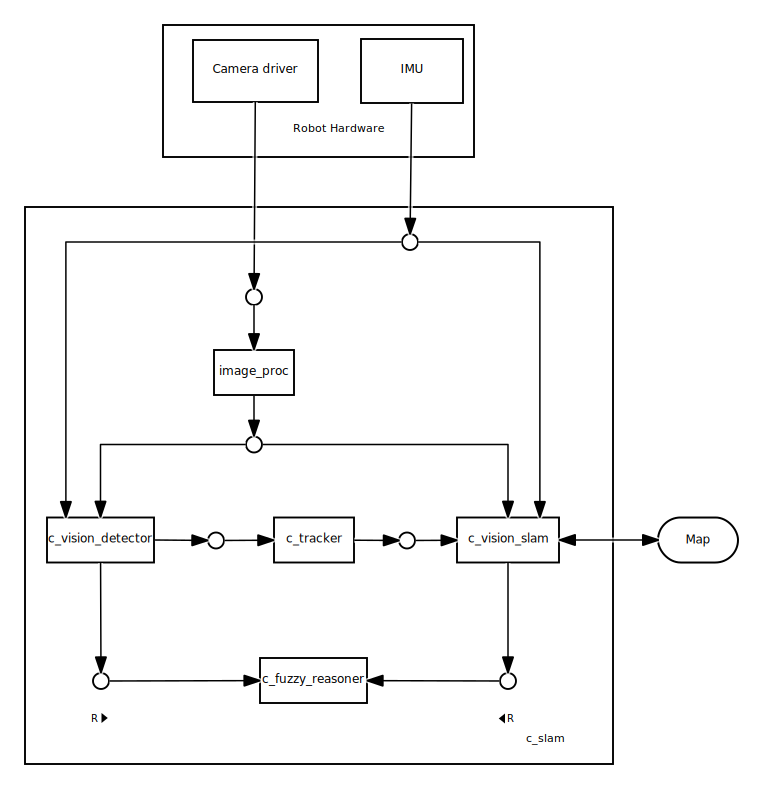
\includegraphics[width=\textwidth]{diagrammi/Sistema}
  \caption{Architettura del sistema implementato}
  \label{fig:architettura-sistema}
\end{figure}


Il diagramma rappresenta i nodi del sistema, segue una breve descrizione di ogni elemento per specificare la loro funzione:

\begin{description}
  \item [image\_proc] si occupa di eliminare la distorsione radiale della videocamera causata dalla curvatura della lente.
  \item [c\_vision\_detector] si occupa di estrarre possibili feature dall'immagine.
  \item [c\_tracking] si occupa di seguire le feature a basso livello estratte dal nodo ``c\_vision\_detector'' nell'immagine, mantenendo un modello in modo da riuscire a riconoscere la feature anche dopo essere stata persa. 
  \item [c\_vision\_slam] si occupa dell'analisi approfondita delle feature, in modo da determinare il tipo di oggetto e la sua posizione nello spazio. 
  \item [c\_fuzzy\_reasoner] implementa un reasoner fuzzy; data una base di conoscenza e un classificatore, analizza le feature in ingresso e le classifica. 
\end{description}


\section{Comunicazione tra i nodi}

Il sistema sviluppato sfrutta per la comunicazione tra i nodi sia il paradigma client-server, per l'interazione con il reasoner, sia il paradigma publish-subscribe, in tutti gli altri casi.
Il reasoner offre 4 servizi:

\begin{description}
 \item [\/reasoning] è un  servizio di reasoning basato su una knowledge base fuzzy
 \item [\/classification] si occupa di classificare istanze di feature riconosciute
 \item [\/getDependencyGraph] restituisce il grafo delle dipendenze del classificatore
 \item [\/getReasoningGraph] restituisce il grafo di reasoning utilizzato dal classificatore
\end{description}

Il reasoner e i suoi servizi verranno discussi approfonditamente  nel \autoref{cap:reasoning}.
%% TODO Se giri i capitoli, saranno stati gia' discussi prima

le informazioni riguardanti gli oggetti riconosciuti e seguiti dal sistema sono scambiate tramite i seguenti topic:

\begin{description}
 \item [\/to\_track] in questo topic vengono pubblicate le possibili feature riconosciute dall'intera immagine. Viene fornito il contorno della feature e la sua possibile classificazione
 \item [\/tracks] in questo topic vengono pubblicati i risultati dell'algoritmo di tracking: contiene il bounding box e il contorno della feature, quest'ultimo viene maggiorato del 20\%, per assicurarsi di mantenere all'interno di esso il reale contorno della feature
\end{description}

Il riconoscimento di feature viene descritto nel \autoref{cap:riconoscimento}, il tracking delle feature riconosciute nel \autoref{cap:tracking}, e infine l'analisi ad alto livello viene effettuata nel \autoref{cap:mapping}.

%% TODO Vd sopra

\section{Parametri degli algoritmi}

Gli algoritmi utilizzati nel sistema, in particolare gli algoritmi di visione, hanno alcuni parametri che è possibile tarare per adattare il sistema a qualsiasi tipo di robot utilizzato.
Per gestire i parametri, abbiamo utilizzato il server dei parametri di ROS.
Il server dei parametri è un dizionario, ossia ogni parametro, identificato da una stringa, è salvato nel server dei parametri, e può essere recuperato tramite il suo nome. 
Il server dei parametri supporta dizionari gerarchici, in modo da poter rappresentare tipi di dati strutturati. 
Inoltre è possibile definire parametri privati per qualsiasi nodo. I parametri privati restano accessibili da tutto il resto del sistema, ma nel dizionario vengono salvati sotto il nome del nodo a cui appartengono; questa caratteristica è fornita per evitare collisioni tra parametri con lo stesso nome in nodi differenti.

Visto che gli algoritmi di estrazione e analisi delle feature si basano fortemente sugli stessi strumenti, il sistema sviluppato usa in maniera estesa i parametri privati, in modo da avere un parametro, che rappresenta concettualmente la stessa quantità, differente per ogni nodo che lo utilizza.

Il sistema permette anche di cambiare i parametri a runtime: essi vengono aggiornati nei nodi che ne fanno uso con una frequenza fissa.
I parametri usati dal sistema e il loro significato sono riportati nell'\autoref{app:manuale}.





\chapter{Reasoning}
\label{cap:reasoning}
\thispagestyle{empty}

\begin{quotation}
{\footnotesize
\noindent \emph{Marty: Aspetta un momento Doc. Se vado dritto verso lo schermo, andrò a sbattere contro quegli indiani! \\
Doc: Marty, non stai pensando quadridimensionalmente!}
\begin{flushright}
Ritorno al Futuro, parte III
\end{flushright}
}
\end{quotation}
\vspace{0.5cm}

\section{Introduzione}

In questo capitolo esporremo il funzionamento del reasoner fuzzy. Il reasoner fuzzzy si basa sulle regole fuzzy descritte da Mamdami~\cite{mamdani1975experiment}. 
Su questa base è stato implementato un classificatore fuzzy ad albero, che, data una struttura ad albero di classi di oggetti e eventuali relazioni tra di loro, accetta in ingresso delle feature, di cui sono note le caratteristiche, e le classifica.
Per raggiungere questo scopo sono stati implementati due linguaggi: uno per esprimere regole fuzzy, che permetta di esprimere le proprietà rispetto a classi di oggetti; l'altro per esprimere la struttura del classificatore, in grado di esprimere gerarchie di classi e relazioni tra esse.
Inoltre è stato implementato un algoritmo di reasoning che permette di classificare un insieme di feature, restituendo non solo le classi a cui ciascuna feature appartiene, ma anche il grado di appartenenza di ciascuna feature alle stesse.
L'algoritmo in particolare è studiato per risolvere dipendenze cicliche tra le classi e riuscire a classificare oggetti che dipendono mutuamente l'uno dall'altro.

\section{Linguaggio Fuzzy}
Il linguaggio per esprimere regole fuzzy sviluppato permette di esprimere non solo domini semplici e insiemi fuzzy su questi domini, ma anche domini complessi, chiamati classi e predicati, validi per qualunque dominio. \`E ispirato fortemente al linguaggio FCL, Fuzzy Control Language, da cui prende parte della sintassi.

Tutte le variabili utilizzate dal reasoner sono assunte come variabili intere con segno, possono quindi avere valori compresi tra \verb|INT_MIN| e \verb|INT_MAX|.
Si assume che i numeri decimali siano rappresentati semplicemente come numeri a virgola fissa.

%%TODO un po' di spiegazione? oppure in concetti fondamentali?

\subsection{Classi e Variabili}
Una classe si definisce tramite la keyword \verb|FUZZIFY_CLASS|, seguita dal nome della classe, e la sua definizione termina con la keyword \verb|END_FUZZIFY_CLASS|.
I fuzzy set riguardanti una variabile di input o output si definiscono tramite la keyword \verb|FUZZIFY|, seguita dal nome della variabile a cui si riferiscono, e terminano con la keyword \verb|END_FUZZIFY|.
Sia le variabili di input che quelle di output possono essere definite all'interno di una classe, così facendo apparterranno alla classe in cui sono definite.
Per definire un fuzzy set, si utilizza una etichetta per definire il nome del fuzzy set, seguito dal token ``:='' e da una etichetta per indicare la sua forma. Ciascuna definizione è terminata dal token ``;''. Le possibili etichette sono:

\begin{description}
 \item [tol] ``Triangle open left'', fuzzy set triangolare aperto a sinistra. Necessita di due parametri.
 \item [tor] ``Triangle open right'', fuzzy set triangolare aperto a destra. Necessita di due parametri.
 \item [tri] ``Triangle'', fuzzy set triangolare. Necessita di tre parametri.
 \item [tra] ``Trapezoid'', fuzy set trapezoidale. Necessita di quattro parametri.
 \item [int] ``Interval'', intervallo. Necessita di due parametri.
 \item [sgt] ``Singleton'', singolo valore. Necessita di un parametro.
\end{description}

I parametri necessari si indicano tra parentesi, separati da virgole.
I nomi delle classi e dei fuzzy set devono cominciare con la lettera maiuscola, mentre i nomi delle variabili possono essere anche minuscoli.


Ad esempio per definire sulla variabile ``Input'' i fuzzy set ``Near'', ``Medium'' e ``Far'' si scrive:

\begin{verbatim}
FUZZIFY Input
 Near := tol(100, 200);
 Medium := tra(100, 200, 300, 400);
 Far := tor(300, 400);
END_FUZZIFY
\end{verbatim}

Mentre per definire una classe chiamata ``TestClass'', con due membri ``a'' e ``b'', si può procedere come segue:

\begin{verbatim}
FUZZIFY_CLASS TestClass
 FUZZIFY a
  Set1 := tol(100, 200);
  Set2 := tra(100, 200, 300, 400);
  Set3 := tor(300, 400);
 END_FUZZIFY
 
 FUZZIFY b
   Fuzzy1 := tol(100, 200);
   Fuzzy2 := tri(100, 200, 300);
   Fuzzy3 := tor(200, 300);
 END_FUZZIFY
END_FUZZIFY_CLASS
\end{verbatim}


\subsection{Regole Fuzzy}
Le regole di Mamdami sono formate da un antecedente e da un conseguente. Nel nostro linguaggio si definiscono tramite le due keyword \verb|IF| e \verb|THEN|.
Dopo il token \verb|IF| ci deve essere una formula logica ben formata, dopo il secondo deve esserci un assegnamento a una variabile.

Una formula ben formata è definita come segue:
\begin{enumerate}
 \item Un assegnamento è una formula ben formata
 \item Un predicato è una formula ben formata
 \item se A è una formula ben formata, anche not A è una formula ben formata
 \item se A e B sono formule ben formate, anche A and B, A or B sono formule ben formate.
 \item null'altyro è una formula ben formata
\end{enumerate}

Un assegnamento di una variabile è composto dal nome della variabile, seguita dalla keyword \verb|IS|, seguita da un fuzzy set da assegnare alla variabile, tutto racchiuso tra parentesi tonde.

Un esempio di regola fuzzy è la seguente:

\begin{verbatim}
if (Input1 is Low) and (Input2 is Medium) then (Output is High); 
\end{verbatim}



\subsection{Predicati}
Si possono anche definire predicati unari. Un predicato unario si definisce tramite la keyword \verb|FUZZIFY_PREDICATE|, seguita dal nome della variabile che si userà nel predicato (che deve necessariamente cominciare con un punto interrogativo). La definizione di un predicato unario termina con la keyword \verb|END_FUZZIFY_PREDICATE|. All'interno di un predicato si devono definire i fuzzy set della variabile usata dal predicato. Più predicati possono essere definiti sulla stessa variabile di input, per farlo basta definire ciauscun predicato con un un nome (che cominci con la lettera maiuscola), seguito dal token ``:='', seguito da una formula logica ben formata, che può usare la variabile di predicato definita, terminata dal token ``;''.

Ad esempio per definire due predicati, ``Predicate1'' e ``Predicate2'', si può procedere come segue:
\begin{verbatim}
FUZZIFY_PREDICATE ?x
 Predicate1 := (?x is Set1) or (?x is Set2);
 Predicate2 := (?x is Set1) and (?x is Set2);
 
 FUZZIFY ?x
   Set1 := tol(0, 100);
   Set2 := tor(0, 100);
 END_FUZZIFY

END_FUZZIFY_PREDICATE
\end{verbatim}

I predicati si chiamano usando il loro nome e aggiungendo tra parentesi la variabile sulla quale si vuole definire il predicato. ad esempio se si vuole valutare il predicato ``Predicate1'' sulla variabile ``a'' si scriverà:
\begin{verbatim}
Predicate1(a)
\end{verbatim}


\subsection{Grammatica}

Segue la grammatica del linguaggio per specificare regole fuzzy.

\begin{tiny}
	\begin{bnf*}
		\bnfprod{fuzzyFile}
			{\bnfpn{fuzzyDefinitions}\bnfsp \bnfpn{ruleSet} } \\
		\bnfprod{fuzzyDefinitions}
			{\bnfpn{fuzzyClass }\bnfpn{fuzzyDefinitions}
			\bnfor \bnfpn{fuzzySet}\bnfsp \bnfpn{fuzzyDefinitions}
			\bnfor \bnfpn{fuzzyPredicate}\bnfsp \bnfpn{fuzzyDefinitions}
			\bnfor \bnfes} \\
		\bnfprod{fuzzyClass}
			{\bnfts{FUZZIFY\_CLASS}\bnfsp \bnftd{ID}\bnfsp \bnfpn{fuzzyClassDefinitions}\bnfsp \bnfts{END\_FUZZIFY\_CLASS}} \\
		\bnfprod{fuzzyClassDefinitions}
			{\bnfpn{fuzzySet}\bnfsp \bnfpn{fuzzyClassDefinitions}
			\bnfor \bnfpn{fuzzyPredicate}\bnfsp \bnfpn{fuzzyClassDefinitions}
			\bnfor \bnfes} \\
		\bnfprod{fuzzyPredicate}
			{\bnfts{FUZZIFY\_PREDICATE} \bnfsp \bnfpn{templateVar}\bnfsp \bnfpn{fuzzyPredicateList} \bnfsp \bnfpn{fuzzyTemplateSet} \bnfsp \bnfts{END\_FUZZIFY\_PREDICATE}} \\
		\bnfprod{fuzzyPredicateList}
			{\bnfpn{fuzzyPredicateDef} \bnfsp \bnfpn{fuzzyPredicateList}
			\bnfor \bnfpn{fuzzyPredicateDef}} \\
		\bnfprod{fuzzyPredicateDef}
			{\bnftd{ID} \bnfsp \bnfts{:=} \bnfsp \bnfpn{wellFormedFormula} \bnfsp \bnfts{;}} \\
		\bnfprod{fuzzyTemplateSet}
			{\bnfts{FUZZIFY} \bnfsp \bnfpn{templateVar} \bnfsp \bnfpn{fuzzyTerm} \bnfsp \bnfts{END\_FUZZIFY}} \\
		\bnfprod{fuzzySet}
			{\bnfts{FUZZIFY} \bnfsp \bnfpn{fuzzyId} \bnfsp \bnfpn{fuzzyTerm} \bnfsp \bnfts{END\_FUZZIFY}} \\
		\bnfprod{fuzzyId}
			{\bnfpn{var}
			\bnfor \bnfpn{var} \bnfsp \bnfts{,} \bnfsp \bnfpn{fuzzyId}} \\
		\bnfprod{fuzzyTerm}
			{\bnftd{ID} \bnfsp \bnfts{:=} F_LABEL \bnfsp \bnfpn{shape} \bnfsp \bnfts{;}
			\bnfor \bnftd{ID} \bnfsp \bnfts{:=} F_LABEL \bnfsp \bnfpn{shape} \bnfsp \bnfts{;} \bnfsp \bnfpn{fuzzyTerm}} \\
		\bnfprod{shape}
			{\bnfts{(} \bnfsp \bnfpn{parametersList} \bnfsp \bnfts{)}} \\
		\bnfprod{parametersList}
			{\bnftd {INTEGER}
			\bnfor \bnftd{INTEGER} \bnfsp \bnfts{,} \bnfsp \bnfpn{parametersList}} \\
		\bnfprod{ruleSet}
			{\bnfpn{rule} \bnfsp \bnfpn{ruleSet}
			\bnfor \bnfes} \\
		\bnfprod{rule}
			{\bnfts{IF} \bnfsp \bnfpn{wellFormedFormula} \bnfsp \bnfpn{fuzzyAssignment} \bnfsp \bnfts{;}} \\
		\bnfprod{wellFormedFormula}
			{\bnfpn{fuzzyComparison}
			\bnfor \bnfpn{fuzzyPredicateCall} 
			\bnfor \bnfts{(} \bnfsp \bnfpn{wellFormedFormula} \bnfsp \bnfts{)}
			\bnfor \bnfts{not} \bnfsp \bnfpn{wellFormedFormula}
			\bnfor \bnfpn{wellFormedFormula} \bnfsp \bnfts{or} \bnfsp \bnfpn{wellFormedFormula}
			\bnfor \bnfpn{wellFormedFormula} \bnfsp \bnfts{and} \bnfsp \bnfpn{wellFormedFormula}} \\
		\bnfprod{fuzzyComparison}
			{\bnfts{(} \bnfsp \bnfpn{variable} \bnfsp \bnfts{IS} \bnfsp \bnftd{ID} \bnfsp \bnfts{)}
			\bnfor \bnfts{(} \bnfsp \bnfsp \bnfsp \bnfpn{templateVar} \bnfsp \bnfsp \bnfsp \bnfts{IS} \bnfsp \bnfsp \bnfsp \bnftd{ID} \bnfsp \bnfsp \bnfsp \bnfts{)}} \\
		\bnfprod{fuzzyPredicateCall}
			{\bnftd{ID} \bnfsp \bnfts{.} \bnfsp \bnftd{ID} \bnfsp \bnfts{(} \bnfsp \bnfpn{variable} \bnfsp \bnfts{)}
			\bnfor \bnftd{ID} \bnfsp \bnfts{(} \bnfsp \bnfpn{variable} \bnfsp \bnfts{)}} \\
		\bnfprod{fuzzyAssignment}
			{\bnfts{THEN} \bnfsp \bnfts{(} \bnfsp \bnfpn{variable} \bnfsp \bnfts{IS} \bnfsp \bnftd{ID} \bnfsp \bnfts{)}} \\
		\bnfprod{variable}
			{\bnftd{ID} \bnfsp \bnfts{.} \bnfsp \bnfpn{var}
			\bnfor \bnfpn{var}} \\
		\bnfprod{var}
			{\bnftd{ID}
			\bnfor \bnftd{VAR\_ID}} \\
		\bnfprod{templateVar}
			{\bnfts{?} \bnfsp \bnfpn{var}} \\
	\end{bnf*}

\end{tiny}




\section{Reasoning}
%%TODO

\section{Linguaggio del classificatore}
%%TODO

\subsection{Grammatica}

\begin{tiny}
	\begin{bnf*}
	\bnfprod{fuzzyClassifiers}
		{\bnfpn{fuzzyClass} \bnfsp \bnfpn{fuzzyClassifiers} \bnfor \bnfpn{fuzzyClass}} \\
	\bnfprod{fuzzyClass}
		{\bnfts{CLASS} \bnfsp \bnftd{ID} \bnfsp \bnfpn{fuzzySuperclass} \bnfsp \bnfpn{hiddenFlag} \bnfsp \bnfpn{fuzzyClassElements} \bnfsp \bnfpn{fuzzyFeatures} \bnfsp \bnfts{END\_CLASS}} \\
	\bnfprod{fuzzySuperclass}
		{\bnfts{EXTENDS} \bnfsp \bnftd{ID} \bnfor \bnfes} \\
	\bnfprod{hiddenFlag}
		{\bnfts{HIDDEN} \bnfor \bnfes} \\
	\bnfprod{fuzzyClassElements}
		{\bnfpn{constants} \bnfsp \bnfpn{variables}
		\bnfor \bnfpn{variables} \bnfsp \bnfpn{constants}
		\bnfor \bnfpn{constants} 
		\bnfor \bnfpn{variables} 
		\bnfor \bnfes} \\
	\bnfprod{constants}
		{\bnfts{CONSTANTS} \bnfsp \bnfpn{constantList} \bnfsp \bnfpn{END\_CONSTANTS}} \\
	\bnfprod{constantList}
		{\bnfpn{var} \bnfsp \bnfts{=} \bnfsp \bnftd{ID} \bnfsp \bnfts{;} \bnfsp \bnfpn{constantList}
		\bnfor \bnfes} \\
	\bnfprod{variables}{\bnfts{VARIABLES} \bnfsp \bnfpn{variableList} \bnfsp \bnfts{END\_VARIABLES}} \\
	\bnfprod{variableList}
		{\bnfpn{var} \bnfsp \bnfts{;} \bnfsp \bnfpn{variableList}
		\bnfor \bnfes} \\
	\bnfprod{fuzzyFeatures}
		{\bnfpn{fuzzyFeature} \bnfsp \bnfts{;} \bnfsp \bnfpn{fuzzyFeatures}
		\bnfor \bnfes} \\
	\bnfprod{fuzzyFeature}
		{\bnfpn{fuzzySimpleFeature}
		\bnfor \bnfpn{fuzzySimpleRelation}
		\bnfor \bnfpn{fuzzyComplexRelation}
		\bnfor \bnfpn{fuzzyInverseRelation}} \\
	\bnfprod{fuzzySimpleFeature}
		{\bnfpn{var} \bnfsp \bnfts{IS} \bnfsp \bnftd{ID}} \\
	\bnfprod{fuzzySimpleRelation}
		{\bnftd{ID} \bnfsp \bnfts{.} \bnfsp \bnfpn{var} \bnfsp \bnfts{MATCH} \bnfsp \bnfpn{var} \bnfsp \bnfpn{fuzzyDegree}} \\
	\bnfprod{fuzzyComplexRelation}
		{\bnftd{ID} \bnfsp \bnfts{.} \bnfsp \bnfpn{var} \bnfsp \bnfpn{fuzzyConstraint} \bnfsp \bnfts{ON} \bnfsp \bnfts{)} \bnfsp \bnfpn{var} \bnfsp \bnfts{,} \bnfsp \bnfpn{var} \bnfsp \bnfts{)}} \\
	\bnfprod{fuzzyInverseRelation}
		{\bnfpn{var} \bnfsp \bnfpn{fuzzyConstraint} \bnfsp \bnfts{ON} \bnfsp \bnftd{ID} \bnfsp \bnfts{)} \bnfsp \bnfpn{var} \bnfsp \bnfts{,} \bnfsp \bnfpn{var} \bnfsp \bnfts{)}} \\
	\bnfprod{fuzzyConstraint}
		{\bnfts{IS} \bnfsp \bnftd{ID}
		\bnfor \bnfes} \\
	\bnfprod{fuzzyDegree}
		{\bnfts{DEGREE} \bnfsp \bnftd{ID}
		\bnfor \bnfes} \\
	\bnfprod{var}
		{\bnftd{ID}
		\bnfor \bnftd{VAR\_ID}} \\
	\end{bnf*}
\end{tiny}



\section{Classificazione}
%%TODO



\chapter{Riconoscimento degli Oggetti}
\label{cap:riconoscimento}
\thispagestyle{empty}

\begin{quotation}
{\footnotesize
\noindent\emph{}
\begin{flushright}
\end{flushright}
}
\end{quotation}
\vspace{0.5cm}


\chapter{Tracking}
\label{cap:tracking}
\thispagestyle{empty}

\begin{quotation}
{\footnotesize
\noindent\emph{Marty: Ma allora dove diavolo sono? \\
Doc: La domanda giusta è: 'Quando diavolo sono?'}
\begin{flushright}
Ritorno al Futuro, parte I
\end{flushright}
}
\end{quotation}
\vspace{0.5cm}

\section{Introduzione}

Una volta riconosciute le possibili feature, è necessario seguirle nelle immagini successive della telecamera.
Per farlo ci siamo basati su un algoritmo presente in letteratura, chiamato Consensus-based Matching and Tracking, CMT~\cite{Nebehay2014WACV}.
L'algoritmo considerato è un algoritmo di tracking a lungo termine. Gli algoritmi di tracking a lungo termine permettono di inseguire oggetti che entrano e escono dal campo visivo della telecamera, e cercano di discriminare anche oggetti simili.

Il tracker implementato è in grado non solo di riconoscere gli oggetti nell'immagine, ma è in grado, in parte, di capire se gli oggetti riconosciuti dall'algoritmo descritto nel \autoref{cap:riconoscimento} sono già o meno nella lista delle track.

In questo capitolo spiegheremo brevemente come funziona l'algoritmo CMT utilizzato e come è stato integrato con il riconoscimento di oggetti e con la costruzione della mappa.

\section{CMT}

L'idea base dell'algoritmo è che i keypoint sono un buon modo per scomporre in parti l'oggetto da seguire. Il primo passo consiste quindi nell'estrarre keypoint dal bounding box iniziale, calcolare i relativi descrittori delle feature e salvare tutto in un database. Questa idea è resa possibile dal recente sviluppo di algoritmi veloci ed efficienti per l'estrazione di feature quali~\cite{rosten_2006_machine} e~\cite{6126542}.

Successivamente, per ogni frame, i keypoint presenti nell'iterazione precedente vengono inseguiti tramite il calcolo del flusso ottico~\cite{Lucas:1981:IIR:1623264.1623280} di Lukas-Kanade, nella variante piramidale~\cite{Bouguet00pyramidalimplementation}. Inoltre vengono estratti keypoint e effettuato il matching con i keypoint presenti nel database. I keypoint di cui è stato effettuato con successo il matching vengono sostituiti a quelli seguiti tramite il flusso ottico, poiché si suppone che siano più stabili, non essendo parte di un processo iterativo di valutazione, soggetto ad errore integrale.

La seconda fase consiste in una procedura di votazione per determinare il centro di massa dell'oggetto.
In primo luogo vengono stimate la scala e la rotazione planare dell'oggetto, calcolando la variazione di scala e di rotazione tra tutte le coppie di keypoint e calcolandone la mediana. In seguito ogni keypoint vota il centro di massa dell'oggetto utilizzando la sua posizione relativa al centro di massa nel primo frame, opportunamente scalato e ruotato grazie ai due valori precedentemente calcolati.

La terza fase dell'algoritmo consiste nell'eliminazione degli outlier tramite un meccanismo di consenso. I centri di massa votati da ciascun singolo keypoint vengono divisi in cluster in base alla distanza euclidea. Quindi, viene individuato il cluster con il maggior numero di voti. Se il cluster scelto ha un numero sufficiente di keypoint, allora l'oggetto viene considerato come visibile e viene calcolato il centro di massa dell'oggetto, eliminando tutti i voti che non appartengono al cluster.

Infine il bounding box dell'oggetto viene calcolato applicando la rotazione e la scala calcolate precedentemente ai punti del bounding box iniziale. Questo procedimento è il punto più debole dell'algoritmo, perché il bounding box calcolato non tiene conto dell'omografia che può esserci tra il bounding box iniziale e quello attuale, causata, ad esempio, dalla distorsione prospettica a seguito della nuova posa della telecamera.

La nostra implementazione si discosta dall'implementazione originale, su cui è fortemente basata, solo per la possibilità di specificare un bounding box con una forma arbitraria.

\section{Integrazione con il riconoscimento degli oggetti}

L'algoritmo di tracking deve essere in grado di interagire con il riconoscimento a basso e alto livello degli oggetti. Per ottenere questo risultato abbiamo implementato alcune euristiche per gestire a basso livello e in maniera semplice i possibili conflitti tra l'algoritmo di tracking e il riconoscimento.

In primo luogo, per facilitare sia il tracking dell'oggetto, sia il riconoscimento ad alto livello, quando il tracker considera un nuovo oggetto da seguire inviato dal riconoscimento a basso livello, non utilizza il bounding box esatto riconosciuto, ma viene maggiorato, scalandolo, in modo da ottenere due importanti risultati:

\begin{enumerate}
 \item Riuscire a riconoscere in maniera efficiente i keypoint che si trovano sui bordi degli oggetti, che spesso sono i keypoint più significativi, soprattutto negli oggetti planari e uniformi, principali obbiettivi di questa tesi.
 \item Riuscire a compensare parzialmente il problema causato dal cambio di posa della telecamera, che potrebbe causare la fuoriuscita dell'oggetto, o parte di esso, dal bounding box, a causa della deformazione prospettica, non calcolata dall'algoritmo.
\end{enumerate}

Le track inviate al riconoscimento di alto livello comprendono due informazioni: il bounding box (maggiorato) e la regione di interesse rettangolare che lo contiene. Questo permette al riconoscimento di alto livello di analizzare solo le regioni di interesse rettangolari dell'immagine, rendendo il compito meno oneroso computazionalmente e di cancellare eventuali feature esterne all'oggetto, che non sono di interesse per il riconoscimento.

L'ultimo problema riguardante l'integrazione, il più problematico, è riuscire a discriminare quali oggetti riconosciuti sono già presenti nella lista delle track.

Questo problema può essere risolto a due livelli. Ad alto livello, è possibile capire che due oggetti trackati nella mappa occupano lo stesso spazio, e quindi fanno parte dello stesso oggetto. Questa soluzione è la soluzione ottimale, ma richiede un maggior numero di informazioni e un costo computazionale maggiore. 
Tuttavia è possibile affrontare parzialmente il problema a basso livello, escludendo in maniera semplice gli oggetti riconosciuti.
L'euristica che abbiamo sviluppato si basa sul calcolo della posizione del centro di massa degli oggetti riconosciuti e delle track, rispetto ai loro bounding box.
Se un oggetto riconosciuto ha il suo centro di massa all'interno di un bounding box di una track attiva, o, viceversa, se una track attiva ha il suo centro di massa nel bounding box dell'oggetto riconosciuto, tale oggetto è considerato già seguito, e non viene aggiunto alla lista delle track.

Come si può vedere dalla figura, %%TODO figura
l'euristica copre abbastanza bene quasi tutti i casi, a parte quando si tratta di oggetti composti da più oggetti o oggetti che si trovano di fronte ad altri oggetti. Per questi casi sono necessarie due ragionamenti ad alto livello differenti: riuscire a capire che un oggetto è semanticamente composto da alcune parti; riuscire a capire che i due oggetti non occupano lo stesso spazio. Per entrambi i ragionamenti non bastano le informazioni estratte dalla singola immagine.

\section{Integrazione con la mappa}
%%TODO non è implementato nulla di quello che c'è scritto in questa sezione. devo toglierlo? l'idea c'è...
L'euristica descritta nel paragrafo precedente dimostra comportarsi molto bene nelle situazioni reali, tuttavia subentrano alcuni problemi quando il tracking degli oggetti presenta dei mancati riconoscimenti. Questo causa spesso la sovrapposizione di più track dello stesso oggetto. Questo problema si può risolvere solamente integrando l'algoritmo di tracking con la mappa degli oggetti riconosciuti. Tramite la mappa è facile accorgersi che lo stesso oggetto è seguito più volte, poiché occupa la stessa posizione dell'oggetto seguito in precedenza.

Il tracking degli oggetti è un compito abbastanza oneroso computazionalmente. Se la posizione del robot è nota, anche in maniera imprecisa, non è necessario mantenere attivo l'algoritmo di tracking per tutti gli oggetti. Inoltre l'algoritmo usato è soggetto a falsi positivi; potendo filtrare le track che non possono essere attive, perché non si trovano nell'area vista dal robot in un determinato istante, il rate di falsi positivi cala drasticamente.

Infine grazie alla stima della posizione, si può calcolare l'omografia che tiene conto della deformazione prospettica del bounding box dell'oggetto rispetto al nuovo punto di vista. Così facendo si può facilitare il riconoscimento ad alto livello.


\chapter{Mapping}
\label{capitolo7}
\thispagestyle{empty}

\begin{quotation}
{\footnotesize
\noindent\emph{}
\begin{flushright}
\end{flushright}
}
\end{quotation}
\vspace{0.5cm}

\chapter{Risultati sperimentali}
\label{capitolo9}
\thispagestyle{empty}

\begin{quotation}
{\footnotesize
\noindent\emph{}
\begin{flushright}
\end{flushright}
}
\end{quotation}
\vspace{0.5cm}

\chapter{Conclusioni e Sviluppi Futuri}
\label{cap:sviluppi}
\thispagestyle{empty}

\begin{quotation}
{\footnotesize
\noindent\emph{}
\begin{flushright}
\end{flushright}
}
\end{quotation}
\vspace{0.5cm}


\cleardoublepage
% ---- Bibliography ----
\bibliographystyle{plain}
\pagenumbering{Roman}
\bibliography{altro/bibliografia}

\appendix

\pagestyle{fancy} 
\fancyfoot{}                                               
\renewcommand{\chaptermark}[1]{\markboth{\appendixname\ \thechapter.\ #1}{}} 
\renewcommand{\sectionmark}[1]{\markright{\thesection.\ #1}}         
\fancyhead[LE,RO]{\bfseries\thepage}    
                                        
\fancyhead[RE]{\bfseries\leftmark}    
\fancyhead[LO]{\bfseries\rightmark}     
\renewcommand{\headrulewidth}{0.3pt} 

\chapter{Il manuale utente}
\label{app:manuale}
\thispagestyle{empty}

\section{Installazione e compilazione}

Per compilare il sistema in maniera completa è necessaria una istallazione completa di ROS. Si veda la guida ufficiale di ROS per conoscere i dettagli dell'istallazione del sistema. \`E necessario utilizzare ROS Hydro Medusa o superiore.  %%TODO link?
Inoltre è necessario installare i generatori di parser Flex e Bison.
\`E possibile compilare la libreria che implementa l'algoritmo di reasoning anche al di fuori di ROS, utilizzando semplicemente CMake. In tal caso si raccomanda di installare anche le librerie Boost.

Una volta installate le dipendenze necessarie, è possibile compilare i sorgenti. Per farlo, create un workspace di catkin, aggiungete i package nella cartella src, e lanciate catkin\_make. Le compilazione avverrà nell'ordine corretto, rispettando le dipendenze tra i package.
\`E necessario aggiungere il file setup.bash nella cartella devel/ del workspace come script da eseguire nel vostro file .bashrc, ad esempio, se il workspace  si chiama catkin\_ws, e si trova nella home, basterà aggiungere al file .bashrc la linea:
source ~/catkin\_ws/devel/setup.bash

Per lanciare i singoli nodi si può utilizzare il programma rosrun. Ricordarsi di aggiungere gli argomenti da linea di comando e i parametri privati necessari subito dopo il nome del package e del nodo che si vuole lanciare. 
I parametri privati vengono specificati aggiungendo un ``\_'' prima del nome del parametro; il cui valore viene assegnato con il token ``:=''.

Ad esempio per lanciare il nodo c\_fuzzy\_reasoner nel package c\_fuzzy si può utilizzare il comando:

rosrun c\_fuzzy c\_fuzzy\_reasoner -c knowledgebase.kb classifier.fuzzy -r knowledgebaseReasoner.kb

Una alternativa per lanciare tutti i nodi contemporaneamente è usare un launchfile. Launchfile di esempio sono presenti nel package c\_slam.

Per lanciare l'intero sistema si può utilizzare il comando:

roslaunch c\_slam c\_slam.launch




\section{Parametri e argomenti}

Di seguito sono elencati e spiegati i parametri utilizzati dai nodi. si veda il \autoref{cap:concetti} per informazioni riguardo agli algoritmi.

\subsection{c\_vision\_detector e c\_vision\_slam}

Questi nodi hanno bisogno necessariamente di parametri privati, senza i quali il loro funzionamento non è garantito.

\subsubsection{Canny}

Questi parametri sono utilizzati dall'algoritmo Canny Edge detector.

\begin{description}
 \item [canny/alpha] rappresenta il valore della soglia bassa, in proporzione alla soglia alta.
 \item [canny/apertureSize] rappresenta la dimensione del kernel con il quale applicare l'operatore di Sobel. Deve essere necessariamente un intero dispari e maggiore o uguale a 3. 
\end{description}

\subsubsection{Hough}

Questi parametri sono utilizzati per l'algoritmo di riconoscimento delle linee, detto trasformata di Hough probabilistica.

\begin{description}
 \item [hough/rho] risoluzione della distanza dall'origine delle rette espressa in pixel.
 \item [hough/teta] risoluzione dell'inclinazione delle rette, espressa in gradi.
 \item [hough/threshold] threshold per l'algoritmo Canny.
 \item [hough/minLineLenght] minima lunghezza delle linee riconosciute, espressa in pixel.
 \item [hough/maxLineGap] massima distanza tra due punti appartenenti alla stessa linea.
\end{description}

\subsubsection{Line filtering}

Questi parametri vengono utilizzati dall'algoritmo che distingue le linee orizzontali e verticali dal rumore.

\begin{description}
 \item [filter/maxDeltaHorizontal] massima inclinazione delle rette orizzontali rispetto alla linea dell'orizzonte.
 \item [filter/maxDeltaVertical] massima inclinazione delle rette verticali rispetto alla linea perpendicolare all'orizzonte.
\end{description}


\subsubsection{Clustering}

Questi parametri servono per tarare il riconoscimento dei cluster. Sono utilizzati dagli algoritmi FAST, per riconoscere i keypoints, e DBSCAN per estrarre da essi i cluster.

\begin{description}
 \item [cluster/threshold] threshold per l'estrazione di keypoints dall'immagine.
 \item [cluster/minPoints] numero minimo di punti necessari a definire un cluster.
 \item [cluster/maxDistance] massima distanza tra i punti di un cluster.
\end{description}

Questi parametri non sono necessari nel nodo c\_vision\_detector.

\subsubsection{classifier}

Questi parametri sono utilizzati dai nodi di visione quando vengono preparate le richieste di reasoning, e quindi sono di fatto utilizzati nel classificatore fuzzy.

\begin{description}
 \item [classifier/threshold] threshold da utilizzare nella classificazione delle feature.
\end{description}

\subsection{c\_fuzzy\_reasoner}

Per lanciare il reasoner è necessario specificare dei parametri da linea di comando.

\begin{description}
 \item [-h] stampa il messaggio di aiuto 
 \item [-r knowledgebase] crea il servizio di reasoning basato sulla knowledgebase specificata.  
 \item [-c knowledgebase classifier] crea il servizio di classificazione a partire dalla knowledgebase e dal classificatore specificati. 

\end{description}


\chapter{Esempio di impiego}
\label{app:esempio}
\thispagestyle{empty}

\noindent Un esempio di impiego del sistema realizzato.

\end{document}
